\documentclass[12]{ctexart}

% base.tex
% ========
% 
% my favorite usepackages and styling.
% `% base.tex
% ========
% 
% my favorite usepackages and styling.
% `% base.tex
% ========
% 
% my favorite usepackages and styling.
% `\input{base.tex}` to import it (before `\begin{document}`).
%

\usepackage{amsmath}
\usepackage{graphicx}
\usepackage{amsfonts}
\usepackage[hidelinks]{hyperref}
\usepackage{url}
\usepackage{algorithm2e}
\usepackage{subcaption}
\usepackage{threeparttable}
\usepackage{booktabs}
\usepackage{listings}
\usepackage{xcolor}


% ================= style =================

% 字号
% \zihao{-5} % 默认字体 -5 五号,-4 小四

% 页边距
% \usepackage{geometry}
% \geometry{a4paper,left=31.8mm,right=31.8mm,top=25.4mm,bottom=25.4mm}

% 页眉页脚
% \pagestyle{plain}

% 小节标题字体
% \ctexset{
%     section = {
%         format = \raggedright\fontsize{13.75pt}{\baselineskip}\bfseries,
%     },
%     subsection = {
%         format = \raggedright\normalsize\bfseries,
%     }
% }

% 算法
\RestyleAlgo{ruled}
% boxed 框(标题在外),boxruled 框(标题在内),ruled 三线, 

% 代码:语法高亮
% https://www.overleaf.com/learn/latex/Code_listing
\definecolor{codegreen}{rgb}{0,0.6,0}
\definecolor{codegray}{rgb}{0.5,0.5,0.5}
\definecolor{codepurple}{rgb}{0.58,0,0.82}
\definecolor{backcolour}{rgb}{0.95,0.95,0.92}
\lstdefinestyle{mystyle}{
    % backgroundcolor=\color{backcolour},   
    commentstyle=\color{codegreen},
    keywordstyle=\color{magenta},
    numberstyle=\tiny\color{codegray},
    stringstyle=\color{codepurple},
    basicstyle=\ttfamily\footnotesize,
    breakatwhitespace=false,
    breaklines=true,
    captionpos=t,
    keepspaces=true,
    numbers=left,
    numbersep=5pt,
    showspaces=false,
    showstringspaces=false,
    showtabs=false,
    tabsize=2,
    flexiblecolumns=t,
    % frame=lrtb,   % 显示边框
}
\lstset{style=mystyle}

\renewcommand{\lstlistingname}{代码}  % Listing -> 代码
\renewcommand{\algorithmcfname}{算法} % Aglorithm -> 代码

% 参考文献样式: 
% https://blog.csdn.net/wy_wy12/article/details/95604258
% \usepackage{gbt7714}
% \bibliographystyle{gbt7714-numerical}
\bibliographystyle{ieeetr}

% =============== end style ===============
` to import it (before `\begin{document}`).
%

\usepackage{amsmath}
\usepackage{graphicx}
\usepackage{amsfonts}
\usepackage[hidelinks]{hyperref}
\usepackage{url}
\usepackage{algorithm2e}
\usepackage{subcaption}
\usepackage{threeparttable}
\usepackage{booktabs}
\usepackage{listings}
\usepackage{xcolor}


% ================= style =================

% 字号
% \zihao{-5} % 默认字体 -5 五号,-4 小四

% 页边距
% \usepackage{geometry}
% \geometry{a4paper,left=31.8mm,right=31.8mm,top=25.4mm,bottom=25.4mm}

% 页眉页脚
% \pagestyle{plain}

% 小节标题字体
% \ctexset{
%     section = {
%         format = \raggedright\fontsize{13.75pt}{\baselineskip}\bfseries,
%     },
%     subsection = {
%         format = \raggedright\normalsize\bfseries,
%     }
% }

% 算法
\RestyleAlgo{ruled}
% boxed 框(标题在外),boxruled 框(标题在内),ruled 三线, 

% 代码:语法高亮
% https://www.overleaf.com/learn/latex/Code_listing
\definecolor{codegreen}{rgb}{0,0.6,0}
\definecolor{codegray}{rgb}{0.5,0.5,0.5}
\definecolor{codepurple}{rgb}{0.58,0,0.82}
\definecolor{backcolour}{rgb}{0.95,0.95,0.92}
\lstdefinestyle{mystyle}{
    % backgroundcolor=\color{backcolour},   
    commentstyle=\color{codegreen},
    keywordstyle=\color{magenta},
    numberstyle=\tiny\color{codegray},
    stringstyle=\color{codepurple},
    basicstyle=\ttfamily\footnotesize,
    breakatwhitespace=false,
    breaklines=true,
    captionpos=t,
    keepspaces=true,
    numbers=left,
    numbersep=5pt,
    showspaces=false,
    showstringspaces=false,
    showtabs=false,
    tabsize=2,
    flexiblecolumns=t,
    % frame=lrtb,   % 显示边框
}
\lstset{style=mystyle}

\renewcommand{\lstlistingname}{代码}  % Listing -> 代码
\renewcommand{\algorithmcfname}{算法} % Aglorithm -> 代码

% 参考文献样式: 
% https://blog.csdn.net/wy_wy12/article/details/95604258
% \usepackage{gbt7714}
% \bibliographystyle{gbt7714-numerical}
\bibliographystyle{ieeetr}

% =============== end style ===============
` to import it (before `\begin{document}`).
%

\usepackage{amsmath}
\usepackage{graphicx}
\usepackage{amsfonts}
\usepackage[hidelinks]{hyperref}
\usepackage{url}
\usepackage{algorithm2e}
\usepackage{subcaption}
\usepackage{threeparttable}
\usepackage{booktabs}
\usepackage{listings}
\usepackage{xcolor}


% ================= style =================

% 字号
% \zihao{-5} % 默认字体 -5 五号,-4 小四

% 页边距
% \usepackage{geometry}
% \geometry{a4paper,left=31.8mm,right=31.8mm,top=25.4mm,bottom=25.4mm}

% 页眉页脚
% \pagestyle{plain}

% 小节标题字体
% \ctexset{
%     section = {
%         format = \raggedright\fontsize{13.75pt}{\baselineskip}\bfseries,
%     },
%     subsection = {
%         format = \raggedright\normalsize\bfseries,
%     }
% }

% 算法
\RestyleAlgo{ruled}
% boxed 框(标题在外),boxruled 框(标题在内),ruled 三线, 

% 代码:语法高亮
% https://www.overleaf.com/learn/latex/Code_listing
\definecolor{codegreen}{rgb}{0,0.6,0}
\definecolor{codegray}{rgb}{0.5,0.5,0.5}
\definecolor{codepurple}{rgb}{0.58,0,0.82}
\definecolor{backcolour}{rgb}{0.95,0.95,0.92}
\lstdefinestyle{mystyle}{
    % backgroundcolor=\color{backcolour},   
    commentstyle=\color{codegreen},
    keywordstyle=\color{magenta},
    numberstyle=\tiny\color{codegray},
    stringstyle=\color{codepurple},
    basicstyle=\ttfamily\footnotesize,
    breakatwhitespace=false,
    breaklines=true,
    captionpos=t,
    keepspaces=true,
    numbers=left,
    numbersep=5pt,
    showspaces=false,
    showstringspaces=false,
    showtabs=false,
    tabsize=2,
    flexiblecolumns=t,
    % frame=lrtb,   % 显示边框
}
\lstset{style=mystyle}

\renewcommand{\lstlistingname}{代码}  % Listing -> 代码
\renewcommand{\algorithmcfname}{算法} % Aglorithm -> 代码

% 参考文献样式: 
% https://blog.csdn.net/wy_wy12/article/details/95604258
% \usepackage{gbt7714}
% \bibliographystyle{gbt7714-numerical}
\bibliographystyle{ieeetr}

% =============== end style ===============


\begin{document}

% ================= title =================

\title{
    重启蒙娜丽莎\bigskip\par
    蔓生都会
}
\author{
    神经漫游者大学 \qquad 赛伯差分机全息玫瑰碎片种植园\\
    蒟蒻蒻 \qquad 666666666666666 \ \ \quad
}

\makeatletter
\renewcommand{\maketitle}{
    \begin{center}
        {\heiti\fontsize{15pt}{\baselineskip}\bfseries\@title}%
        \bigskip\par\noindent
        {\songti\normalsize\@author}%
        \bigskip\par\noindent
    \end{center}
}
\makeatother

\maketitle

% =============== abstract ===============

{\noindent\bfseries{摘要}}:
本文展示了一个简单报告的模版,基于 CTeX \cite{ctex}等宏包进行排版。本文旨在提供算法、代码、三线表、图片、双图并排等常用语法实例。

{\noindent\bfseries{关键词}}:
镜子,朝闻道,时间移民,微纪元

% \setcounter{section}{-1} % 从 0 开始编 section 号

% =============== content ===============

\section{概述}

银河系西旋臂少人问津的末端,未经勘测的荒僻区域深处,有一颗无人理睬的小小黄色恒星。

以约莫九千两百万英里半径绕其旋转的,是一颗彻底无关紧要的小小蓝绿色行星,这里从\emph{猿猴}繁衍而来的生命形式原始得让人吃惊,居然还以为\emph{数字式电子表}是什么很高明的主意。

这颗行星有(更确切的说法: 曾经有)一个问题,那就是: 星球上的绝大多数居民在绝大多数时间里都不开心。针对这个问题提出过许多解决方案,但绝大多数方案基本上都和某种绿色小纸片的流动相关,这可真是怪事一桩,因为从头到尾不开心的又不是绿色小纸片。

于是乎,问题依然如故;很多人类过得一塌糊涂,其中大部分更是生不如死,连戴数字式电子表的也不例外。

% 很多人越来越认为,当初从树上下来已是大错特错。有些人甚至说连上树这一步都不对,一开始就不该离开海洋。

% 如此这般,距离某君因为说大家都该换换思路、与人为善而被钉在树上约两千年后的某个星期四,有位姑娘独自坐在里克曼沃斯的小咖啡馆里,忽然领悟到一直以来究竟是哪儿出了岔子,终于知道了怎样把这个世界变成和谐欢乐的好地方。这次的解决方案很正确,能成功,也不会有人被钉在任何东西上。

% 可令人悲哀的是,在她有机会找到电话告诉别人之前,一场恐怖而愚蠢的大灾难陡然降临,她的想法因此永远湮灭。

% 这是她的故事。

\section{设计与实现}

可以借助 VS Code + \LaTeX\ Workshop 编译该文档,如附录 \ref{appendix_a} 所示。

\subsection{文本}
 
随着四散迸溅的旋律,一个色彩变幻不定的小球渐渐胀大,在半空中爆裂成众多不规则的团块\cite{sklearn},一起盘旋而上,然后迅速下落,如同相互交错的弧形彩带\cite{movielens}。那些团块又凝聚成无数颗小珠子,每颗的色彩都不尽相同——这时候,\emph{贝泰}开始看出一点名堂了:
\begin{equation}
    b_{ui} = \mu+b_u+b_i
\end{equation}

她发现如果闭起眼睛,彩色的图案 $u$ 反而更加清晰\cite{surprise};每颗彩珠的每个小动作 $i=i(u)$ 都带着特有的节奏;她还发现自己竟然无法确认这些色彩;此外彩珠其实并非珠状,而是许多小小的人形。 

用 \verb$\verb|...|$ 可以写句内的等宽代码,如果代码内要有竖线(\verb$|$),则可以把定界符 \verb$|$ 替换为 \verb|$|。

\subsection{算法 \label{knn} }

算法块由 algorithm2e 宏包\cite{algorithm2e}实现,排版效果如算法 \ref{algo_recom} 所示。

\begin{algorithm}[H]
    \caption{一种朴素的推荐算法}
    \label{algo_recom}

    \SetKwInOut{Input}{Input}
    \SetKwInOut{Data}{Data}
    \SetKwInOut{Output}{Output}

    \Input{user $u_i \in U$}
    \Data{objects $\forall o_j \in O$}
    \Output{recommended objects $o'_0, \cdots, o'_k$}

    $u \leftarrow embedding(u_i)$\;

    \For{$o_j \in O$}{
        $o \leftarrow embedding(o_j)$\;
        $r_{i,j} \leftarrow ranking(u, o)$\;
    }

    $O' \leftarrow sorted(\forall o_j \in O$ by $r_{i,j})$\;
    return $\{o'_0, \cdots, o'_k\} \subseteq  O'$\;
\end{algorithm}

\subsection{枚举}

\begin{enumerate}
    \item 海伯利安\\
    第八届世界未来学大会在哥斯达黎加举行。说实话,要不是塔兰托加教授明确指示我必须参加这个会议,我根本不会去纽纳斯那种地方。

    \item 海伯利安的陨落(后面刻意加了大空行:)\\

    \item 安迪密恩

    \item 安迪密恩的觉醒

\end{enumerate}

\subsection{代码}

代码块使用 listings 宏包\cite{listings}实现。配置了等宽小字体,支持多种语言的基本语法高亮,如代码 \ref{lst_code} 所示。

\begin{lstlisting}[language=Python, caption={Python example}, label={lst_code}]
import numpy as np
    
def incmatrix(genl1,genl2):
    m = len(genl1)
    n = len(genl2)
    M = None #to become the incidence matrix
    VT = np.zeros((n*m,1), int)  #dummy variable
    
    #compute the bitwise xor matrix
    M1 = bitxormatrix(genl1)
    M2 = np.triu(bitxormatrix(genl2),1) 

    for i in range(m-1):
        for j in range(i+1, m):
            [r,c] = np.where(M2 == M1[i,j])
            for k in range(len(r)):
                VT[(i)*n + r[k]] = 1;
                VT[(i)*n + c[k]] = 1;
                VT[(j)*n + r[k]] = 1;
                VT[(j)*n + c[k]] = 1;
                
                if M is None:
                    M = np.copy(VT)
                else:
                    M = np.concatenate((M, VT), 1)
                
                VT = np.zeros((n*m,1), int)
    
    return M
\end{lstlisting}

\section{实验}

\subsection{表格}

如表 \ref{tab_emotextBenchmark} 所示。该表格语法较为复杂,是由于引入了宽度缩放(tabcolsep)、表格注释(threeparttable)、三线表(toprule、midrule、bottomrule)等诸多特性的缘故,在实际的使用中,可以按需删减。

\begin{table}[!ht]
    \centering
    \setlength{\tabcolsep}{8mm}{
        \caption{某种带有注释的三线表}
        \label{tab_emotextBenchmark}
        \begin{threeparttable}
            \begin{tabular}{cccc}
                \toprule
                Loops       & Time                & sec per loop & Mem     \\
                \midrule
                0\tnote{*}  & -                   & -            & 132.9MB \\
                1\tnote{**} & 0.731               & 0.7314       & 194.8MB \\
                10          & 0.646               & 0.0646       & 171.8MB \\
                100         & 6.227               & 0.0623       & 171.8MB \\
                1000        & 69.22               & 0.0692       & 171.8MB \\
                % \hline
                % 测试环境        & \multicolumn{3}{l}{
                %     Intel(R) Core(TM) i5-7360U CPU @ 2.30GHz
                % }                                                          \\
                % ~           & \multicolumn{3}{l}{
                %     Python 3.9.9 (main, Nov 21 2021, 03:23:44)
                % }                                                          \\
                % ~           & \multicolumn{3}{l}{
                %     [Clang 13.0.0 (clang-1300.0.29.3)] on darwin
                % }                                                          \\
                \bottomrule
            \end{tabular}
            \begin{tablenotes}
                \footnotesize
                \item[*] 这是一个注释。
                \item[**] 这是表格的另一个注释。
            \end{tablenotes}
        \end{threeparttable}
    }
\end{table}

\subsection{单图片}

插入图片如图 \ref{fig_lstm} 所示,推荐图片导出为 PDF 格式,PDF 在这里引用进来之后是可以选中里面的文字的,非常 fancy。

\begin{figure}[h!tbp]
    \centering
    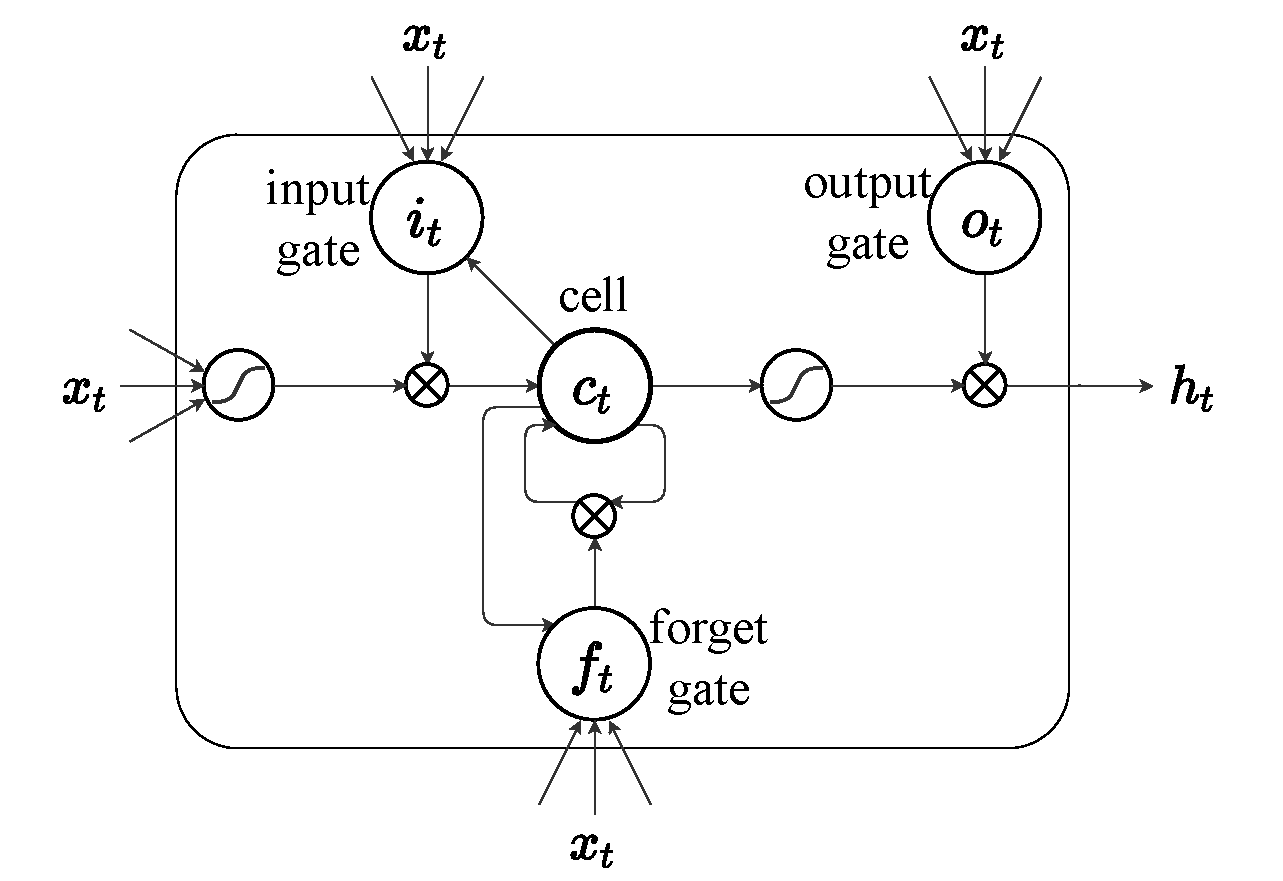
\includegraphics[width=0.8\linewidth]{imgs/lstmCell.pdf}
    \caption{一个关于 LSTM 的图片}
    \label{fig_lstm}
\end{figure}

如果 $\mathtt{width=0.8 \backslash linewidth}$ 的写法超出纸张了,也可以尝试用 $\mathtt{scale=0.6}$ 之类的缩放语法。

\subsection{双图并排}

一种简单的双图并排排版如图 \ref{fig_two} 所示。其中值得注意的是,这里的 subfigure 以及里面的 includegraphics 的宽度设置就非常玄学,不同的图片需要手动调整,多做尝试。

\begin{figure}[!ht]
    \begin{subfigure}[t]{0.48\linewidth}
        \centering
        
\includegraphics[width=0.9\linewidth]{imgs/TODO.pdf}
        \caption{左边的子图}
        \label{fig_subfig_1}
    \end{subfigure}
    % \hspace{0.8cm}
    \begin{subfigure}[t]{0.48\linewidth}
        \centering
        
\includegraphics[width=0.9\linewidth]{imgs/TODO.pdf}
        \caption{右边的子图}
        \label{fig_subfig_2}
    \end{subfigure}
    \caption{并排的两个图片}
    \label{fig_two}
\end{figure}

\section{结论}

星星逐渐稀疏,银河耀目的光亮也暗淡下来,逐渐从他相逢过的灿烂光华,化为一种淡淡的魅光——但是将来等他准备好之后,会再度与那灿烂光华相逢。

他精确地回到自己想去的那个地方——那个人类称之为真实的空间。

% =============== appendix ===============

\newpage

\appendix

\section{附录: 参考的编译设置}\label{appendix_a}

\begin{lstlisting}[language=Go, caption={适用于 VS Code + LaTeX Workshop 的编译设置}, label={lst_vscode}]
    "latex-workshop.latex.recipes": [
        {
          "name": "xelatex -> bibtex -> xelatex × 2",
          "tools": ["xelatex", "bibtex", "xelatex", "xelatex"]
        },
    ],
    "latex-workshop.latex.tools": [
        {
          "name": "xelatex",
          "command": "xelatex",
          "args": [
            "--shell-escape", 
            "-synctex=1", 
            "-interaction=nonstopmode", 
            "-file-line-error", 
            "%DOC%"
          ],
          "env": {}
        },
        {
          "name": "bibtex",
          "command": "bibtex",
          "args": ["%DOCFILE%"],
          "env": {}
        }
    ]
\end{lstlisting}

% =============== bibliography ===============

\newpage

% \ctexset{
%     section = {
%       format = \normalsize\bfseries\centering,
%      }
% }
\bibliography{references.bib}

\end{document}
